\documentclass[11pt]{article}
\usepackage[review]{acl}
\usepackage{times}
\usepackage{latexsym}
\usepackage[T1]{fontenc}
\usepackage[utf8]{inputenc}
\usepackage{microtype}
\usepackage{inconsolata}
\usepackage{graphicx}
\usepackage{amsmath}
\usepackage{booktabs}
\usepackage{placeins}
\graphicspath{{figures/}}

\title{Cooperation Is Not One Number: Scaffold, Group Size, and Persistence\\in Repeated Social Dilemmas Among LLM Agents}
\author{Anonymous submission}

\begin{document}
\maketitle

\begin{abstract}
A single cooperation score hides three quantities: how much an LLM agent cooperates, how cooperation changes with group size, and whether it lasts. We measure all three in 376 episodes of repeated homogeneous self-play across six models and group sizes $N=2$--$5$. Two prompts differ only in a constant ranking of immediate payoffs that favors defection. The ranking lowers cooperation in all six models, to at most 6.75\% with it, while free-form levels range from 2.72\% to 80.24\%. Mistral drops from 80.24\% to 6.75\% and per-seat reward falls from 6.57 to 0.13, yet its group-size response is statistically uncertain. Only Llama's group-size interaction ($+14.02$ points) survives six-model Holm correction, and a pooled decline with group size is not supported. Cooperation also need not persist: DeepSeek's free-form cooperation falls from 39.87\% in rounds 1--5 to 2.79\% in rounds 26--30, with streak breaks at median round 3 and terminal zero cooperation at median round 24, without establishing a causal end-game effect. Execution failures, most visibly for Qwen, further shape what trajectories mean. Our reporting checklist separates cooperation level, group-size response, and persistence, with episode-level uncertainty, the exact payoff presentation, and fallback rates.
\end{abstract}

\section{Introduction}
Cooperation scores are increasingly used to characterize LLM agents \citep{akata2025repeated,fontana2025nicer,vallinder2025cultural}. A typical evaluation runs agents through a social dilemma and reports average cooperation, sometimes as a function of group size. This single number conflates three distinct quantities: the \emph{level} of cooperation, the \emph{group-size response} (how cooperation changes as more agents are added), and \emph{persistence} (whether early cooperation survives later rounds). Because LLM agents act on textual descriptions of incentives, histories, and actions, each of these quantities can also depend on how the task is presented and on whether the execution pipeline returns valid actions.

We study these quantities in one repeated graded cooperation game, holding the environment fixed. We run 376 fresh episodes of homogeneous self-play across six models, $N\in\{2,3,4,5\}$, and two prompt scaffolds. Both scaffolds give the same state, histories, long-term reward objective, and output schema. The \emph{structured} scaffold additionally lists a constant ranking of immediate action payoffs, which always favors defection; the \emph{free-form} scaffold omits it. The contrast therefore isolates the salience of immediate incentives; it is not a comparison of reasoning against no reasoning.

\paragraph{Findings.}
\begin{itemize}
\item \textbf{Presentation changes levels in every model; group size does so inconsistently.} With the ranking, every model's cooperation is at most 6.75\%; without it, levels range from 2.72\% to 80.24\%. Free-form--structured gaps range from 2.5 to 73.5 points (median 13.5), driven largely by Mistral (73.5 points, with per-seat reward falling from 6.57 to 0.13).

\item \textbf{Group-size responses are model-specific.} Interactions are heterogeneous across models ($Q(5)=18.23$, $p=.0027$, $I^2=72.6\%$). Only Llama's survives Holm correction. The proposed pooled decline of cooperation with group size is not supported here.
\item \textbf{Early cooperation need not persist.} DeepSeek falls from 39.87\% to 2.79\% between rounds 1--5 and 26--30. Its first streak breaks occur at median round 3 and often recover, while terminal zero cooperation begins at median round 24; Mistral stays at 78--80\%. The horizon is disclosed, so end-game reasoning is possible, but the timing does not establish it.
\item \textbf{Execution reliability constrains interpretation.} Fallback actions are full defection, so pipeline failures bias behavior toward defection. Qwen's trajectories illustrate this most clearly.
\end{itemize}

\paragraph{Contributions.} (i) A controlled group-size-by-scaffold evaluation with episode-level uncertainty. (ii) A model-resolved decomposition of cooperation into level, group-size response, and persistence, showing that these can dissociate. (iii) An execution-reliability analysis identifying where pipeline behavior limits what cooperation scores mean. (iv) A concrete reporting checklist for evaluating cooperation in LLM agents (Section~\ref{sec:recs}). We do not propose a universal scaling law or a communication mechanism; the claims concern this environment, these checkpoints, and these prompts.

\begin{table*}[t]
\centering\small
\begin{tabular}{lrrrrr}
\toprule
Model & S level (\%) & F level (\%) & $D_m$ (pp) & F rounds 1--5 (\%) & F rounds 26--30 (\%) \\
\midrule
Llama & 6.52 & 20.43 & +14.02 & 23.41 & 21.94 \\
Qwen & 0.14 & 6.24 & -3.91 & 22.57 & 0.00 \\
Gemma & 0.00 & 13.02 & -5.79 & 13.53 & 17.02 \\
Mistral & 6.75 & 80.24 & -6.81 & 78.08 & 80.30 \\
DeepSeek & 1.19 & 18.24 & +5.73 & 39.87 & 2.79 \\
GPT-OSS & 0.26 & 2.72 & -7.87 & 12.54 & 0.00 \\
\bottomrule
\end{tabular}
\caption{Cooperation is not one number: levels, group-size responses, and persistence describe different behavior. S/F denote structured/free-form. Levels and early/late cooperation average equally across four group sizes; the early/late comparison is descriptive. $D_m$ is the endpoint-scale difference between fitted free-form and structured group-size slopes, not a raw endpoint difference. Table~\ref{tab:main-h4} reports its uncertainty and adjusted tests. Qwen's values describe the tested execution pipeline (Section~\ref{sec:reliability}).}
\label{tab:measurement-grid}
\end{table*}


\section{Related Work}
\label{sec:related}
\paragraph{LLMs in repeated games and game-theoretic evaluation.}
\citet{akata2025repeated} evaluate cooperation and coordination in finitely repeated two-player games, while \citet{fontana2025nicer} study the iterated Prisoner's Dilemma against adversaries with different defection rates. \citet{vallinder2025cultural} examine indirect reciprocity across generations of LLM agents in a Donor Game. Broader game-theoretic evaluations probe rationality and strategic reasoning across distinct games \citep{fan2024rational,duan2024gtbench}.
\citet{piatti2024cooperate} study sustainable cooperation in societies of LLM agents, and \citet{piedrahita2025corrupted} examine free-riding by reasoning-focused models in public-goods games with costly sanctioning. These works place cooperation within interacting agent populations. We instead hold one environment fixed and ask which conclusions follow from levels, fitted group-size responses, and trajectories.
Relative to the two-player and cultural-evolution settings above, our design jointly examines group size and an immediate-payoff presentation scaffold in one fixed environment, separating cooperation level, persistence, and execution reliability; this is a difference in evaluation design, not a claim to introduce repeated-game or prompt-based evaluation \citep{akata2025repeated,fontana2025nicer,vallinder2025cultural}.

\paragraph{Group size, public goods, and cooperative AI.}
Classical work shows that cooperation need not decline monotonically with group size; the relationship depends on benefit scaling and saturation \citep{scirep2015groupsize,plos2015curvilinear}, and extends to spatial and reinforcement-learning settings \citep{szolnoki2012spatial,rsos2024rlpgg}. These studies motivate specifying payoff aggregation before interpreting a group-size response. Here, benefits depend on the \emph{average} cooperation of others rather than their sum.
\citet{isaac1988groupsize} distinguish group number from marginal return in public-goods provision, finding no pure numbers-in-the-group effect in their experiment. Classical work studies reciprocity in repeated interaction \citep{axelrod1981cooperation} and the role of costly punishment in sustaining public-goods contributions \citep{fehr2000punishment}. Sequential social dilemmas extend cooperation from atomic actions to learned policies \citep{leibo2017sequential}, while cooperative AI frames capabilities and tools for mutually beneficial interaction as a broader research agenda \citep{dafoe2020cooperative}.

\paragraph{Prompt sensitivity and evaluation validity.}
Meaning-preserving formatting choices can change few-shot model performance \citep{sclar2024formatting}, and instruction paraphrases can change both absolute and relative performance \citep{mizrahi2024multiprompt}. Few-shot evaluations can also be unstable across prompt formats and example orders \citep{zhao2021calibrate}. These findings motivate documenting presentation choices, without establishing the mechanism of our payoff-ranking effect. Benchmark design must also be assessed against the abilities it is intended to measure \citep{bowman2021benchmarking}.
\citet{goodyear2025state} show that state representation affects LLM-agent behavior in dynamic routing games, and MAgIC evaluates social abilities across social-deduction and game-theoretic scenarios \citep{xu2024magic}. Our intervention adds an immediate-payoff ranking while retaining state, histories, objectives, and output schema, and we measure its association with levels and group-size responses separately. We do not propose new metrics; the contribution is the joint, model-resolved evaluation under a documented intervention.

\section{The Environment}
\label{sec:env}
We use a repeated $N$-player graded cooperation game with endogenous payoff dynamics and an optional perception-noise mechanism, fixed to zero here. At each round $t$, every player $i$ simultaneously selects $a^t_i \in \{0,\dots,M-1\}$, mapped to a cooperation level
\begin{equation}
  c^t_i = 1 - \frac{a^t_i}{M-1},
\end{equation}
so $a=0$ is full cooperation and $a=M-1$ is full defection. Player $i$'s reward is
\begin{equation}
  u^t_i = B^t_{\text{eff}} \cdot \bar{c}^t_{-i} - C \cdot c^t_i + K,
\end{equation}
where $\bar{c}^t_{-i} = \frac{1}{N-1}\sum_{j \neq i} c^t_j$ is the \emph{average} cooperation of the other $N-1$ players. At fixed $B^t_{\text{eff}}$, benefits do not mechanically grow with $N$. A player's own cooperation incurs an immediate cost without directly raising their own current reward; its contribution to each other player's average is scaled by $1/(N-1)$, and to the public group mean by $1/N$. These facts specify the aggregation rule, but endogenous future benefits prevent them from determining a repeated-game group-size effect on their own.

Two endogenous mechanisms shape $B^t_{\text{eff}}$: a public cooperation streak amplifies the benefit through a saturating bonus when group cooperation exceeds $\theta$, and a slower drift process adjusts the base benefit using recent cooperation (recurrences in Appendix~\ref{sec:env-recurrences}).

\section{Experimental Design}
\label{sec:design}
\subsection{Models, Conditions, and Replication}
We test Llama-3.1-8B-Instruct, Qwen3-8B, Gemma-3-12B-IT, Mistral-Small-3.1-24B-Instruct, DeepSeek-R1-Distill-Qwen-14B, and GPT-OSS-120B. The roster is purposive and spans developers; it is not a controlled parameter-scale sweep or a set of independent training lineages (DeepSeek's checkpoint is distilled onto a Qwen base). DeepSeek and GPT-OSS form a designated exploratory reasoning group; because Qwen3 also supports thinking \citep{qwen32025}, this is not a comprehensive capability taxonomy.

All seats in an episode share model and condition. The 48 cells cross six models, four group sizes, and two modes, with $M=5$, noise $p=0$, threshold $\theta=.50$, and $T=30$ rounds. Fresh seeds per cell are unequal (2--16): 14/4/8/3/16/2 in the roster order above, balanced across each model's eight cells, for 376 episodes and 39{,}480 seat-round decisions. Pilot episodes were used for planning and are excluded from all main results (Appendix~\ref{sec:appendix-amendment}).

The environment fixes $B_0=12$, $C=8$, $K=0$, $B_t\in[9,15]$, drift window 8, $\eta=.35$, reference cooperation .55, streak threshold .50, bonus scale $\lambda=.25$, and saturation $\tau=4$. Observation histories contain at most ten prior rounds; agents have history-only memory, no opponent-prediction output, and no inter-agent communication. When the pipeline returns no valid decision, it supplies a fallback action (full defection; Section~\ref{sec:reliability}). The prompt discloses the horizon: all 39{,}480 saved agent inputs contain both $T=30$ and the number of rounds remaining, so end-game reasoning is available in both scaffolds \citep{selten1986end}.

\paragraph{Scaffolds.}
Both prompts ask agents to maximize their own long-term average reward, consider immediate and future consequences, and return the same JSON schema. Structured play additionally receives a ranking by $\mathrm{score}(a)=-C\,c(a)$. The opponent-benefit term cancels when comparing one's own actions, so the ranking is always $[4,3,2,1,0]$ with scores $[0,-2,-4,-6,-8]$, independent of $N$, state, and history. Agents are explicitly free to reject the top-ranked action. The ranking omits future streak and drift benefits, although both modes receive their rules. Full prompts are in the appendix; serving details are in Appendix~\ref{sec:execution}.

\subsection{Measurements}
The unit of analysis is the episode. The primary outcome is mean normalized cooperation across all seats and all 30 rounds. Reward, terminal streak, and terminal benefit are secondary; first-attempt parse and fallback rates are reliability metrics. We report three separate measurements:
\begin{itemize}
\item \textbf{Level:} episode-mean cooperation per model and scaffold, averaged equally over the four group sizes.
\item \textbf{Group-size response:} within each model, the endpoint-scale scaffold-by-$N$ interaction $D_m=3(\beta_{\mathrm{free},m}-\beta_{\mathrm{struct},m})$, where $\beta$ is the fitted cooperation slope per added player. Positive $D_m$ means a more positive group-size response in free-form play; it does not imply higher cooperation at every $N$. We report marginal and six-model Holm-adjusted tests, plus an inverse-variance heterogeneity test (Appendix~\ref{sec:analysis-details}).
\item \textbf{Persistence:} cooperation in rounds 1--5 versus 26--30, descriptively; no temporal significance test is claimed.
\end{itemize}
Two pooled tests complement the within-model analysis. The first (H1) tests a negative structured-condition slope over $N$ in a Gaussian mixed model with model-level random intercept and $N$ slope. The second (H2) compares a flat model with a dilution model $a+b/(N-1)$ in structured episodes by AIC/BIC. The pooled mixed-model interaction is secondary and descriptive. The within-model interaction analysis (H3) was made primary by a dated internal amendment before main data collection; this is not an external preregistration (Appendix~\ref{sec:appendix-amendment}).

\section{Results}
\label{sec:results}
All 376 planned episodes completed and enter the primary analysis. Ten of 48 cells have zero observed episode variance; these floors constrain detection without establishing deterministic policies.

\subsection{Level: The Ranking Pushes Every Model Toward Defection}
\textbf{Free-form mean cooperation exceeds structured mean cooperation in all six models} (Table~\ref{tab:main-h4}; full outcomes in Appendix~\ref{sec:outcomes}). Mistral is the clearest case: 80.24\% cooperation free-form versus 6.75\% structured, a 73.5-point gap, with mean per-seat reward of 6.57 versus .13. This compares whole interacting populations, not the payoff of one agent switching against fixed opponents. Gemma shows the extreme of the structured condition: zero cooperation in every structured episode (Figure~\ref{fig:main-coop}). Group-size effects are less consistent: the only interaction that survives correction is 14.02 points (below), and the pooled structured slope over $N$ is not distinguishable from zero ($-0.04$ points per added player, 95\% CI $[-1.76,1.68]$). Individual free-form cells can still change sharply with $N$ (Gemma falls from 30.91\% at $N=4$ to 0\% at $N=5$), so the claim is about the typical size of the two effects in this environment, not that group size never matters. Free-form--structured gaps across the six models range from 2.5 to 73.5 points (Appendix~\ref{sec:outcomes}). Gap size tracks the free-form baseline, since the ranking cannot suppress cooperation that is already near zero. Llama's surviving interaction ($+14.02$) is comparable to its own level gap (13.9), so we do not claim that scaffold effects exceed group-size effects in every model: the scaffold lowers cooperation in all six, while group-size responses are model-specific.

\begin{figure*}[t]
\centering
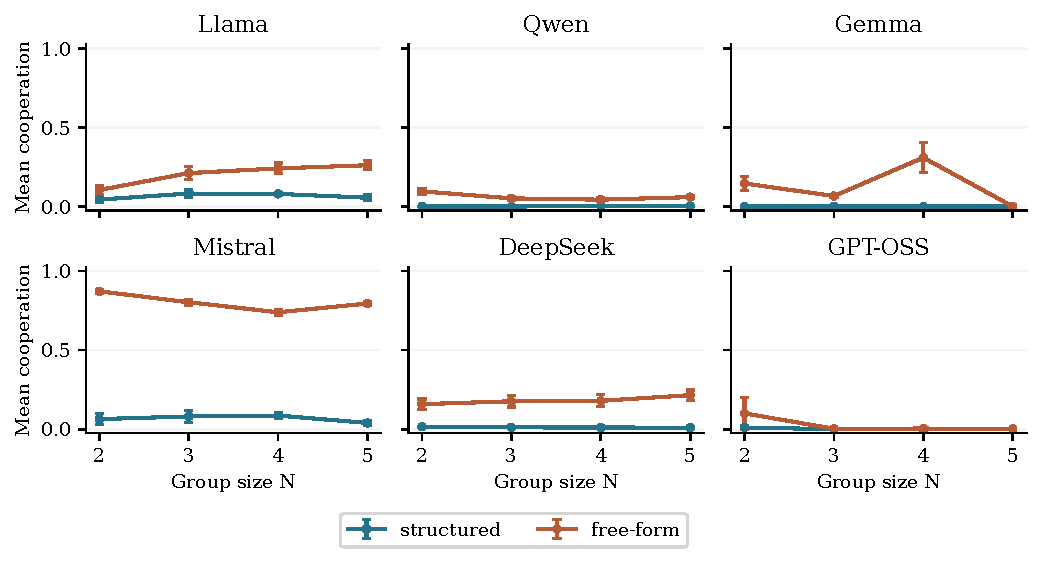
\includegraphics[width=\textwidth]{main_cooperation.pdf}
\caption{Complete main cooperation by group size and scaffold. Points are cell episode means; bars are one standard error across independent episodes. Seats and rounds are not treated as independent replicates. Floor values and non-monotonic responses qualify a universal scaling-decline account.}
\label{fig:main-coop}
\end{figure*}

\subsection{Group-Size Response: Model-Specific and Mostly Uncertain}
\begin{table*}[t]
\centering
\small
\setlength{\tabcolsep}{3pt}
\begin{tabular}{lrrrrrrr}
\toprule
Model & S coop. & F coop. & $s_m$ & $D_m$ (pp) & 95\% CI & $p$ & Holm $p$ \\
\midrule
Llama & 6.52 & 20.43 & 14 & +14.02 & [4.67, 23.37] & 0.004 & 0.024 \\
Qwen & 0.14 & 6.24 & 4 & -3.91 & [-8.54, 0.73] & 0.084 & 0.421 \\
Gemma & 0.00 & 13.02 & 8 & -5.79 & [-16.11, 4.52] & 0.247 & 0.623 \\
Mistral & 6.75 & 80.24 & 3 & -6.81 & [-16.93, 3.31] & 0.151 & 0.602 \\
DeepSeek & 1.19 & 18.24 & 16 & +5.73 & [-3.32, 14.78] & 0.208 & 0.623 \\
GPT-OSS & 0.26 & 2.72 & 2 & -7.87 & [-116.99, 101.24] & 0.542 & 0.623 \\
\bottomrule
\end{tabular}
\caption{Large scaffold-associated level gaps need not imply supported group-size interactions. S/F denote structured/free-form; cooperation is mean normalized cooperation in percent, averaged equally over four group sizes; $s_m$ is seeds per cell. $D_m$ is the free-form-minus-structured fitted linear cooperation change from $N=2$ to $N=5$ in percentage points, using all four group sizes. Intervals use eight-cell Welch uncertainty; Holm adjustment covers all six model tests. Only Llama's interaction survives correction.}
\label{tab:main-h4}
\end{table*}

A large level gap does not imply a group-size interaction. Mistral's interaction is $-6.81$ points (95\% CI $[-16.93,3.31]$), despite its 73.5-point level gap. Across the six models, interactions are heterogeneous: $Q(5)=18.23$, $p=.0027$, $I^2=72.6\%$. Only Llama survives six-model Holm correction: its interaction is $+14.02$ points (95\% CI $[4.67,23.37]$, marginal $p=.004$, Holm $p=.024$). Free-form cooperation rises from 10.42\% at $N=2$ to 26.10\% at $N=5$, while structured cooperation changes from 4.37\% to 5.54\%. All other individual intervals include zero.

GPT-OSS's interval is uninformative: two seeds per cell yield Welch degrees of freedom 1.02 and an untruncated interval of $[-116.99,101.24]$ points. We keep GPT-OSS in the analysis but draw no conclusions from its interaction.

\paragraph{Pooled tests.}
The secondary pooled mixed-model interaction is $+4.04$ points (95\% CI $[-2.72,10.80]$, $p=.242$); it is descriptive and lacks a model-specific random interaction slope. The pooled slope test (H1) is not supported: the structured-reference $N$ coefficient is $-0.040$ percentage points per added player (95\% CI $[-1.764,1.684]$, $p=.964$). The dilution comparison (H2) is not supported either: the flat model has AIC $-602.03$ and BIC $-595.56$, versus $-600.29$ and $-590.58$ for dilution, and the dilution coefficient $b=-.00616$ has the opposite sign to the proposed decline. The commonly assumed pooled decline of cooperation with group size is not supported in this environment. Gemma's free-form means are non-monotonic across $N$ (14.53\%, 6.63\%, 30.91\%, 0\%), a shape that linear slopes conceal.

\paragraph{Sensitivity to the least reliable models.} Because Qwen has low first-attempt parse rates and GPT-OSS has two seeds per cell, we repeated the heterogeneity test and Holm correction post hoc without Qwen, and without Qwen and GPT-OSS. Excluding Qwen gives $Q(4)=15.46$, $p=.0038$, $I^2=74.1\%$; excluding both gives $Q(3)=14.47$, $p=.0023$, $I^2=79.3\%$. Llama's interaction remains the only significant interaction after Holm correction in each reduced family (Holm $p=.020$ and $.016$). This check is post hoc and does not replace the planned six-model analysis.

\subsection{Persistence: Early Cooperation Need Not Last}
\label{sec:persistence}
Mistral's free-form cooperation persists, from 78.08\% in rounds 1--5 to 80.30\% in rounds 26--30. Others do not (Figure~\ref{fig:dynamics}): DeepSeek's free-form average falls from 39.87\% to 2.79\%, and GPT-OSS has zero cooperation throughout the last five rounds in every free-form episode (with only two seeds per cell). Qwen's recorded free-form opening-round cooperation is 59.11\%, yet every free-form episode has zero cooperation throughout rounds 26--30; because of Qwen's low first-attempt extraction success, we treat this as a pipeline-level trajectory rather than a clean strategic finding (Section~\ref{sec:reliability}). Early cooperation and persistence are therefore separate measurements: an episode average or an opening-round score would rank DeepSeek and Qwen much higher than their late behavior warrants.

\paragraph{Post-hoc event timing.}
Saved inputs expose both $T=30$ and rounds remaining in all 39{,}480 decisions.
In DeepSeek free-form play, 56/64 episodes have an active streak break
(group-mean cooperation $g_t<.5$ after a positive streak), with first breaks at median round 3;
36/56 return to $g_t\geq.5$ within the next three rounds. A break therefore
need not be permanent collapse. Defining terminal zero cooperation as an all-zero suffix through round 30, 59/64 DeepSeek free-form episodes enter this state, at median round 24; 24/59 onsets fall in rounds 26--30, so most onsets (35/59) precede the final five rounds. Qwen enters terminal zero cooperation in 16/16 free-form episodes, at median round 18, with no onsets in the last five rounds; because of its pipeline confounds (Section~\ref{sec:reliability}), this timing is not a clean strategic observation. Mistral does so in 0/12. These timings distinguish early breaks from terminal decline, and the disclosed horizon makes end-game reasoning available, but they do not identify a causal end-game effect (Appendix~\ref{sec:log-descriptions}). Group-size-specific trajectories (Figure~\ref{fig:traj-by-N}, Appendix~\ref{sec:app-viz}) show DeepSeek's free-form decline and Mistral's free-form persistence across $N$.

\paragraph{Returned explanations.}
In Mistral play, literal ranking keywords occur in 1{,}067/1{,}260 structured explanations (84.7\%) versus 0/1{,}260 free-form explanations, so the added ranking is visibly salient to the agents. Explicit horizon keywords occur in 294/1{,}260 structured (23.3\%) and 352/1{,}260 free-form explanations (27.9\%), so horizon mentions are not specific to either scaffold. These exploratory text counts describe what is mentioned; they neither validate the explanations nor reveal hidden reasoning (Appendix~\ref{sec:log-descriptions}). Mistral free-form mentions the horizon in 27.9\% of explanations yet stays at 78.08\%--80.30\% cooperation from rounds 1--5 through 26--30, so horizon mentions need not coincide with end-game defection (mentions and actions are not aligned by construction).

\begin{figure*}[t]
\centering
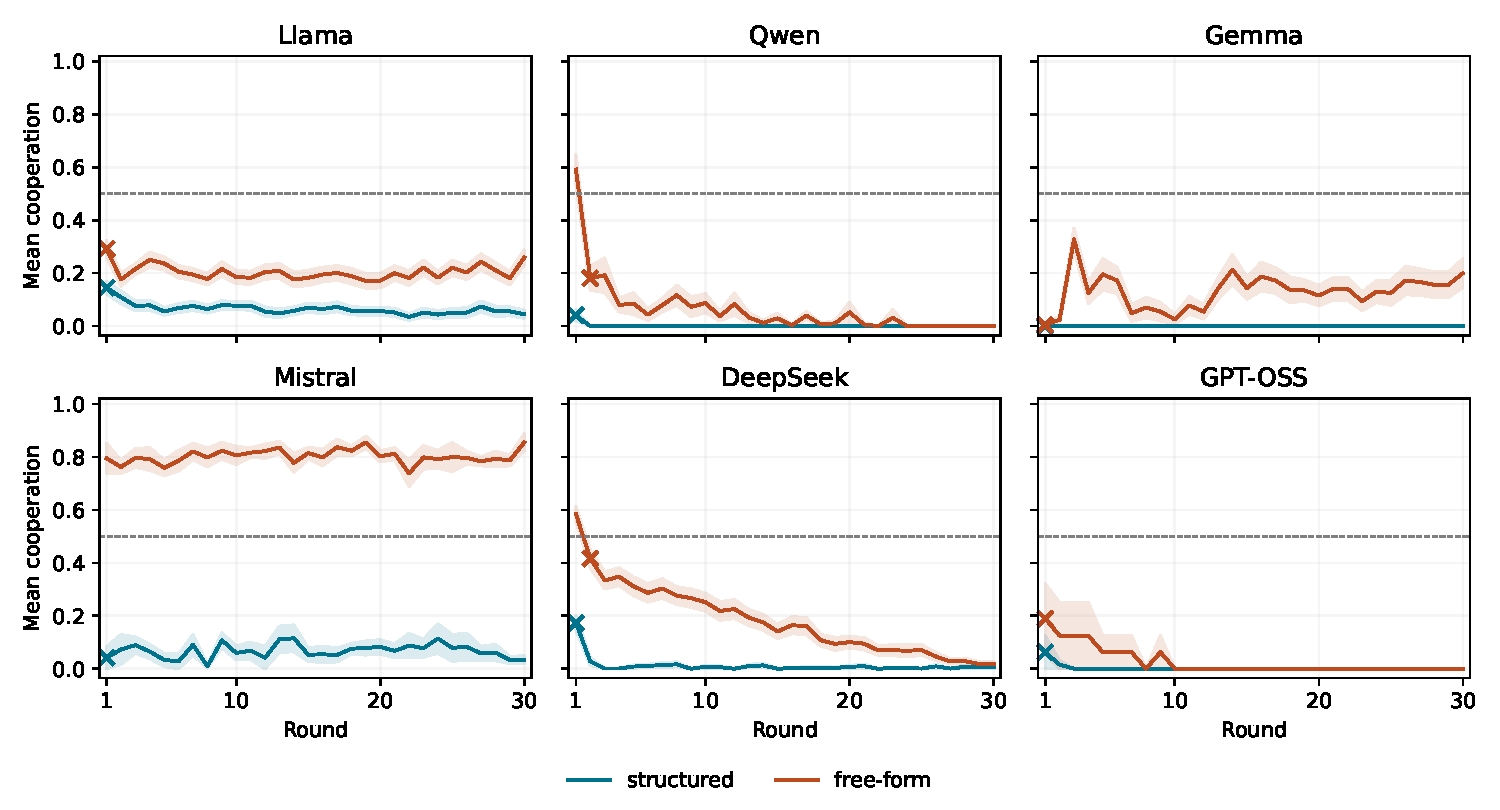
\includegraphics[width=\textwidth]{main_dynamics.pdf}
\caption{Cooperation trajectories averaged equally across four group sizes. Shading is one standard error of the stratified mean computed from independent episode trajectories. The dashed line marks $\theta=.5$; crosses mark the first model--scaffold mean below it, including round-1 values. An aggregate crossing is not an episode streak reset. Actual active-break and terminal-zero timings are reported separately in Appendix~\ref{sec:log-descriptions}. Group-size-specific trajectories appear in Figure~\ref{fig:traj-by-N}.}
\label{fig:dynamics}
\end{figure*}

\subsection{Execution Reliability: What a Cooperation Score Includes}
\label{sec:reliability}
Every one of the 48 cells passes the 12\% fallback ceiling fixed before main collection (maximum observed cell rate 7\%), and the primary analysis retains fallback-affected trajectories (Table~\ref{tab:main-reliability}). The fallback action is full defection (action 4; Appendix~\ref{sec:env-recurrences}), so fallbacks bias affected decisions toward defection rather than acting as a neutral default.

Qwen is the clearest case. Fallbacks occur on 0/1{,}680 structured and 100/1{,}680 free-form decisions (6.0\%). A post-hoc saved-log check finds no fallbacks in its final five free-form rounds (0/280 decisions), all of which have zero cooperation, so late defection is not direct fallback substitution. Earlier fallback-affected histories can still shape later behavior, so strategy cannot be cleanly separated from execution for Qwen (Appendix~\ref{sec:qwen-log-check}). Qwen's extraction errors are dominated by unterminated thinking blocks (Appendix~\ref{sec:execution}), consistent with an output-budget bottleneck. We therefore read Qwen's trajectory as a demonstration of why execution reliability must be reported, not as evidence about Qwen's strategic disposition.

Other models: Gemma has no fallbacks, so its 3{,}360 structured defections cannot be attributed to the fallback rule. DeepSeek has 0.03\%/0.10\% structured/free-form fallback, Llama 0.4\%/1.3\%, and GPT-OSS 0.0\%/0.7\%. These rates characterize the tested pipeline, not intrinsic ability. Exploratory E1 finds no clean separation of interaction directions between the designated reasoning group and the other models (Appendix~\ref{sec:e1}).

\section{Recommendations for Evaluating Cooperation}
\label{sec:recs}
Our results suggest a reporting checklist for studies of cooperation in LLM agents.
\begin{enumerate}
\item \textbf{Report the exact scaffold and payoff representation.} A constant ranking of immediate payoffs lowered cooperation in all six models (by 73.5 points for Mistral) without changing any rule.
\item \textbf{Report level and group-size response separately, per model, with episode-level uncertainty.} Level gaps and slope interactions dissociate, and pooled estimates hide heterogeneity ($I^2=72.6\%$).
\item \textbf{Report round trajectories and event timing, and state whether the horizon is disclosed.} Opening or episode-mean cooperation can look high when late-round cooperation is near zero, and whether agents know the horizon changes how late collapse can be read.
\item \textbf{Report fallback rates and the fallback action.} A defecting fallback silently contributes to measured defection.
\item \textbf{State replication per cell and treat floors carefully.} Unequal seeds and zero-variance cells limit what null results mean.
\end{enumerate}

\section{Discussion and Conclusion}
A cooperation score characterizes a model operating through a specified prompt and execution pipeline; it is not an intrinsic cooperative disposition. In one repeated game across six models, the presentation of immediate payoffs lowered cooperation in every model, sharply for Mistral, group-size responses were model-specific (only Llama's survived correction), the pooled decline with group size was not supported, and early cooperation often disappeared. Evaluations should therefore report levels, group-size responses, and trajectories separately, with episode-level uncertainty and execution reliability. Explaining \emph{why} agents defect, whether through diluted accountability, reciprocity, threshold coordination, or horizon reasoning, requires controls we leave to future work: frozen benefits, opponent matching, and a hidden-horizon condition. Our timing analysis shows that early streak breaks often recover and that terminal zero cooperation usually begins well before the last five rounds for DeepSeek, which any such account must accommodate.

\section*{Limitations}
\paragraph{Scope.} This is a single English-language game with homogeneous self-play, $N\le5$, 30 rounds, one temperature, no communication, and no human baseline. The ranking is constant and myopic and omits future benefits; the scaffold contrast evaluates this particular presentation, not structured reasoning in general. There is no frozen-benefit or opponent-matching ablation, so mechanisms are not identified. Returned explanations are not hidden reasoning \citep{turpin2023unfaithful,lanham2023faithfulness}. We make no claims about morality, universal reasoning-model behavior, or the causal mechanism behind cooperation. The horizon is disclosed to agents and there is no hidden-horizon condition, so end-game reasoning cannot be separated from other sources of late defection.

\paragraph{Models and statistics.} The six checkpoints are a purposive sample with overlapping lineages, and parameter count is confounded with architecture, training, and serving. Replication is unequal (2--16 seeds per cell), and H1/H2 weight models unequally. Power-aware design and reporting experimental details alongside scores are established concerns in NLP evaluation \citep{card2020power,dodge2019reporting}. The $Q$ test has only five degrees of freedom and uncertain estimated variances. Welch uncertainty is weak for GPT-OSS. The pooled Gaussian model has floor-heavy outcomes and a boundary warning; convergence does not validate its distributional assumptions. Null individual results do not exclude smaller effects, and planned marginal power is not family-wise power. The heterogeneity test is not included in the six-test Holm correction. Comparing a level gap with an interaction slope is a comparison of different quantities on a common percentage-point scale, not a formal test of relative magnitude.

\paragraph{Execution.} Passing the fallback gate does not remove fallback influence. Qwen was run with a 2{,}048-token output ceiling versus 8{,}192 for DeepSeek, and most of its extraction errors contain unterminated thinking blocks; the reported Qwen episode cohort uses this original budget, and its trajectories are pipeline-confounded. Parse success does not guarantee action validity, and hardware and token ceilings vary across models. Main and pilot parsers differ for five models, so variance transport from pilot to main is uncertain. Temporal observations are descriptive, not confirmatory. Streak breaks are defined from cooperation itself, and event-conditioned summaries cannot establish a causal effect of a break. Terminal-zero onsets depend on the observed horizon and do not distinguish backward induction from other dynamics. Keyword rules are unvalidated literal text matches; omissions and paraphrases can be missed, and mentions need not agree with actions.

\section*{Ethical Considerations}
The experiment uses simulated agent interactions and no human participants or personal data. Cooperation and defection are operational action labels, not moral judgments or evidence of real-world intent. The results do not establish general trustworthiness.

\section*{Data and Code Availability}
The appendix provides prompts, environment recurrences, serving configuration, and analysis specification. Code and experiment logs are not publicly released with this submission, which limits independent verification.

\bibliography{custom}
\appendix

\section{Pilot-Informed Design and Internal Amendments}
\label{sec:appendix-amendment}
The 240-episode pilot has five seeds per cell, $T=30$, temperature .7 and top-$p=1.0$. Eleven cells have zero observed variance. The original extractor applies to five pilot models; GPT-OSS uses final-decision v2. All fresh main data use v2 and no pilot outcomes are credited.

On 7 October 2026, an internal amendment made within-model interactions and heterogeneity primary for the interaction analysis (H3); the pooled interaction (H3) became secondary/descriptive. H1/H2 were unchanged. Hypothesis labels H1--H3 follow the numbering of our internal records after an early candidate hypothesis was dropped before data collection. A compute amendment replaced a 10-point/90\% marginal-power proposal with a 15-point target, a 25\% variance margin and the allocation below; the 29-chunk schedule changes ownership of execution only. These are dated internal records, not an external preregistration. The compute-constrained allocation does not imply 90\% power for every model or simultaneous detection of all six effects.
\begin{table}[t]
\centering
\small
\setlength{\tabcolsep}{4pt}
\begin{tabular}{lrrrr}
\toprule
Model & $s_m$ & Episodes & Target $s_m$ & Power \\
\midrule
Llama & 14 & 112 & 20 & 76.9\% \\
Qwen & 4 & 32 & 4 & 96.0\% \\
Gemma & 8 & 64 & 11 & 75.6\% \\
Mistral & 3 & 24 & 3 & 94.4\% \\
DeepSeek & 16 & 128 & 23 & 77.6\% \\
GPT-OSS & 2 & 16 & 2 & 100.0\% \\
\bottomrule
\end{tabular}
\caption{Authorized fresh main allocation. Target replication is the plug-in requirement for 90\% marginal power at a 15-point endpoint interaction with pilot variances inflated by 25\%. Power is prospective at the allocated replication, not achieved power or simultaneous six-test power.}
\label{tab:allocation}
\end{table}

\begin{table}[t]
\centering
\small
\setlength{\tabcolsep}{4pt}
\begin{tabular}{lrrr}
\toprule
Model & $\widehat D_m$ (pp) & Endpoint (pp) & Zero-var. cells \\
\midrule
Llama & +21.91 & +22.22 & 0 \\
Qwen & -7.79 & -8.55 & 3 \\
Gemma & -8.69 & -9.00 & 5 \\
Mistral & -2.32 & -3.25 & 0 \\
DeepSeek & +8.55 & +9.83 & 0 \\
GPT-OSS & +0.25 & +0.25 & 3 \\
\bottomrule
\end{tabular}
\caption{Pilot only: fitted endpoint interaction versus literal endpoint sensitivity. Positive values mean that free-form cooperation changes more positively from $N=2$ to $N=5$ than structured cooperation. Each model has eight cells with five seeds each. These are design-review summaries, not main-study hypothesis tests.}
\label{tab:pilot}
\end{table}

The six pilot fitted interactions have sample variance .0134210 (squared proportion units), based on only five variance degrees of freedom. A population sensitivity gives a non-shrinking variance floor of $.0134210/6$. Infinite-seed normal power ceilings are 18.46\%, 56.14\% and 88.72\% at 5/10/15 points; a noncentral-$t$ sensitivity with five degrees of freedom gives 13.95\%, 40.27\% and 71.85\%. These planning calculations are not main-data achieved power and do not match a fitter lacking random interaction heterogeneity. GPT-OSS's main contrast variance coefficient is .01638 versus .0000934 in the pilot, so pilot-based precision did not transport to the small main sample; we did not use the realized effect to choose additional replication.

\paragraph{Pooled-model diagnostics.} The pooled fit converged using L-BFGS with the planned random intercept and $N$ slope; an MLE boundary warning remains. No fitted prediction lies outside $[0,1]$. We retain the planned specification without post-hoc respecification. The mixed model has an intercept-only fallback if no usable converged fit is obtained, and no episode random intercept is added to an episode-mean outcome.

\section{Execution and Reliability}
\label{sec:execution}
Local vLLM endpoints use temperature .7 and top-$p=1.0$. DeepSeek's output ceiling is 8{,}192 tokens; all others use 2{,}048. Context limit is 16{,}384 and tensor parallelism one. Jobs use H100/H200 GPUs; GPT-OSS uses H200 with MXFP4 weights. Tables~\ref{tab:serving} and~\ref{tab:main-reliability} report actual serving and reliability. The 29 single-GPU chunks consumed 141.29 allocated GPU-hours (132.38 hours of recorded episode execution), spanning 58.17 hours from first allocation start to last finish.

All 29 scheduled study jobs completed. Worker logs record vLLM 0.25.1, PyTorch 2.11.0 and Transformers 5.14.1. Activation dtype is bfloat16. GPU inventory was recorded, but peak VRAM was not measured. Latencies cover the complete decision pipeline and reflect actual hardware assignments, not a standardized speed benchmark.
\begin{table*}[t]
\centering
\small
\setlength{\tabcolsep}{4pt}
\begin{tabular}{lrrllrr}
\toprule
Model & Tokens & GPU & Dtype & Quant. & S sec. & F sec. \\
\midrule
Llama & 2048 & H100/H200 & bfloat16 & -- & 0.99 & 1.40 \\
Qwen & 2048 & H100/H200 & bfloat16 & -- & 15.71 & 26.02 \\
Gemma & 2048 & H100/H200 & bfloat16 & -- & 1.32 & 1.48 \\
Mistral & 2048 & H100/H200 & bfloat16 & -- & 3.71 & 3.69 \\
DeepSeek & 8192 & H100/H200 & bfloat16 & -- & 20.11 & 33.41 \\
GPT-OSS & 2048 & H200 & bfloat16 & MXFP4 & 7.50 & 9.15 \\
\bottomrule
\end{tabular}
\caption{Actual main serving configuration and mean end-to-end decision latency. All jobs use TP=1, context limit 16,384, vLLM 0.25.1, torch 2.11.0 and transformers 5.14.1. No peak-VRAM time series was recorded.}
\label{tab:serving}
\end{table*}

\begin{table*}[t]
\centering
\small
\setlength{\tabcolsep}{4pt}
\begin{tabular}{llrrrr}
\toprule
Model & Mode & Decisions & Parse (\%) & Fallback (\%) & Seconds \\
\midrule
Llama & S & 5880 & 95.5 & 0.4 & 0.99 \\
Llama & F & 5880 & 89.7 & 1.3 & 1.40 \\
Qwen & S & 1680 & 31.5 & 0.0 & 15.71 \\
Qwen & F & 1680 & 7.9 & 6.0 & 26.02 \\
Gemma & S & 3360 & 100.0 & 0.0 & 1.32 \\
Gemma & F & 3360 & 100.0 & 0.0 & 1.48 \\
Mistral & S & 1260 & 98.8 & 0.0 & 3.71 \\
Mistral & F & 1260 & 99.4 & 0.0 & 3.69 \\
DeepSeek & S & 6720 & 99.3 & 0.0 & 20.11 \\
DeepSeek & F & 6720 & 97.9 & 0.1 & 33.41 \\
GPT-OSS & S & 840 & 93.5 & 0.0 & 7.50 \\
GPT-OSS & F & 840 & 83.3 & 0.7 & 9.15 \\
\bottomrule
\end{tabular}
\caption{Fresh-main reliability. Parse is recomputed using the actual v2 extractor, not the historical proxy; it does not imply action validity. Fallback uses the original flags. Seconds are mean end-to-end decision latency. Seat-round rates are descriptive; all 48 cells satisfy the 12\% fallback gate.}
\label{tab:main-reliability}
\end{table*}

First-parse rates are recomputed with the actual v2 extractor; raw historical proxy flags remain preserved. JSON extraction success does not guarantee action validity. Among Qwen's 3{,}664 extraction errors, 3{,}417 contain an unterminated thinking block. This is consistent with an output-budget bottleneck, but the client did not retain finish reasons or token usage, so truncation cannot be established for every case.

\section{Analysis Details}
\label{sec:analysis-details}
Within each model, the interaction analysis (H3) uses a linear-in-$N$ regression with mode and their interaction. The endpoint-scale estimand is
\begin{equation}
 D_m=3\bigl(\beta_{\mathrm{free},m}-\beta_{\mathrm{struct},m}\bigr),
\end{equation}
where the $\beta$'s are the respective linear-in-$N$ slopes. All four $N$ levels contribute; this is not the literal two-endpoint difference. With cell episode variance $v_{m,r,N}$ and $s_m$ seeds per cell,
\begin{equation}
 \begin{aligned}
 q_m&=\sum_{r,N}[0.6(N-3.5)]^2v_{m,r,N},\\
 \mathrm{Var}(\widehat D_m)&=q_m/s_m.
 \end{aligned}
\end{equation}
The endpoint multiplier gives weights $3(N-3.5)/5=0.6(N-3.5)$; the mode contrast has opposite signs, which disappear on squaring. The implementation combines OLS point estimates with cell-specific variances and Welch--Satterthwaite $t$ uncertainty \citep{welch1947variances}. Main-data variances are re-estimated; pilot variances are planning inputs only. We report two-sided marginal $p$-values at $\alpha=.05$ and supplemental Holm-adjusted $p$-values \citep{holm1979sequential}.

The heterogeneity analysis (H3) uses inverse-variance weights $w_m$ and $Q=\sum_m w_m(\widehat D_m-\bar D_w)^2$, with the approximate $\chi^2_5$ reference and $I^2=\max(0,(Q-5)/Q)$ (zero when $Q=0$), using the $I^2$ summary of \citet{higgins2002heterogeneity}. Six models and estimated standard errors limit calibration. A significant $Q$ indicates heterogeneity, not a proof of inadequate power. The post-hoc sensitivity analyses use the same estimator and standard errors with the specified model subset removed; Holm corrections are recomputed within each reduced family using the reported marginal $p$-values.

\section{Complete Descriptive Outcomes}
\label{sec:outcomes}
Table~\ref{tab:main-outcomes} preserves all cooperation, early/late and reward summaries, including columns omitted from the main results anchor.
\begin{table*}[t]
\centering
\small
\setlength{\tabcolsep}{4pt}
\begin{tabular}{lrrrrrr}
\toprule
Model & S coop. & F coop. & F early & F late & S reward & F reward \\
\midrule
Llama & 6.52 & 20.43 & 23.41 & 21.94 & 0.16 & 0.63 \\
Qwen & 0.14 & 6.24 & 22.57 & 0.00 & 0.01 & 0.23 \\
Gemma & 0.00 & 13.02 & 13.53 & 17.02 & 0.00 & 0.49 \\
Mistral & 6.75 & 80.24 & 78.08 & 80.30 & 0.13 & 6.57 \\
DeepSeek & 1.19 & 18.24 & 39.87 & 2.79 & 0.04 & 0.84 \\
GPT-OSS & 0.26 & 2.72 & 12.54 & 0.00 & 0.01 & 0.15 \\
\bottomrule
\end{tabular}
\caption{Descriptive main outcomes averaged equally over the four N cells. Cooperation is percent; early/late are rounds 1--5/26--30. Reward is per seat per round. These summaries add no confirmatory tests.}
\label{tab:main-outcomes}
\end{table*}


\section{Exploratory Reasoning-Group Comparison}
\label{sec:e1}
The designated reasoning group shows no clean separation of interaction directions: DeepSeek is positive, GPT-OSS negative; Llama is positive and the other three models negative. The exploratory status--direction correlation is .25 (Fisher exact $p=1.0$). This small, confounded grouping cannot identify an effect of reasoning training.

\section{Environment Recurrences and Execution Seeds}
\label{sec:env-recurrences}
Let $g_t=N^{-1}\sum_i c_i^t$, $s_0=0$ and $B_1=12$. The current payoff uses
\begin{equation}
 B_{\mathrm{eff}}^t=B_t[1+.25\tanh(s_{t-1}/4)].
\end{equation}
After actions, $s_t=s_{t-1}+1$ if $g_t\geq.5$ and zero otherwise. Let $r_t$ be the average of the available $g$ values over the last eight rounds including $t$. Drift updates
\begin{equation}
 B_{t+1}=\mathrm{clip}_{[9,15]}[B_t+.35(r_t-.55)].
\end{equation}
With zero perception noise, observed cooperation means are true means. The base benefit is bounded by 15; the streak-amplified effective benefit can exceed 15. Observations expose current benefit, streak, rolling state, prior ten-round action histories and action frequencies, never simultaneous current opponent actions. Generation seeds are derived from phase, episode identity (including condition) and seat, so equal episode seed labels across modes do not imply paired random generations. Fallback maximizes $-C\,c(a)$ with a cooperative tie-break; at $C=8$ its unique choice is action~4 (full defection).

\section{Additional Main Visualizations}
\label{sec:app-viz}
Figure~\ref{fig:traj-by-N} separates the group-size-averaged trajectories of the main text by $N$ and scaffold.
\begin{figure*}[t]
\centering
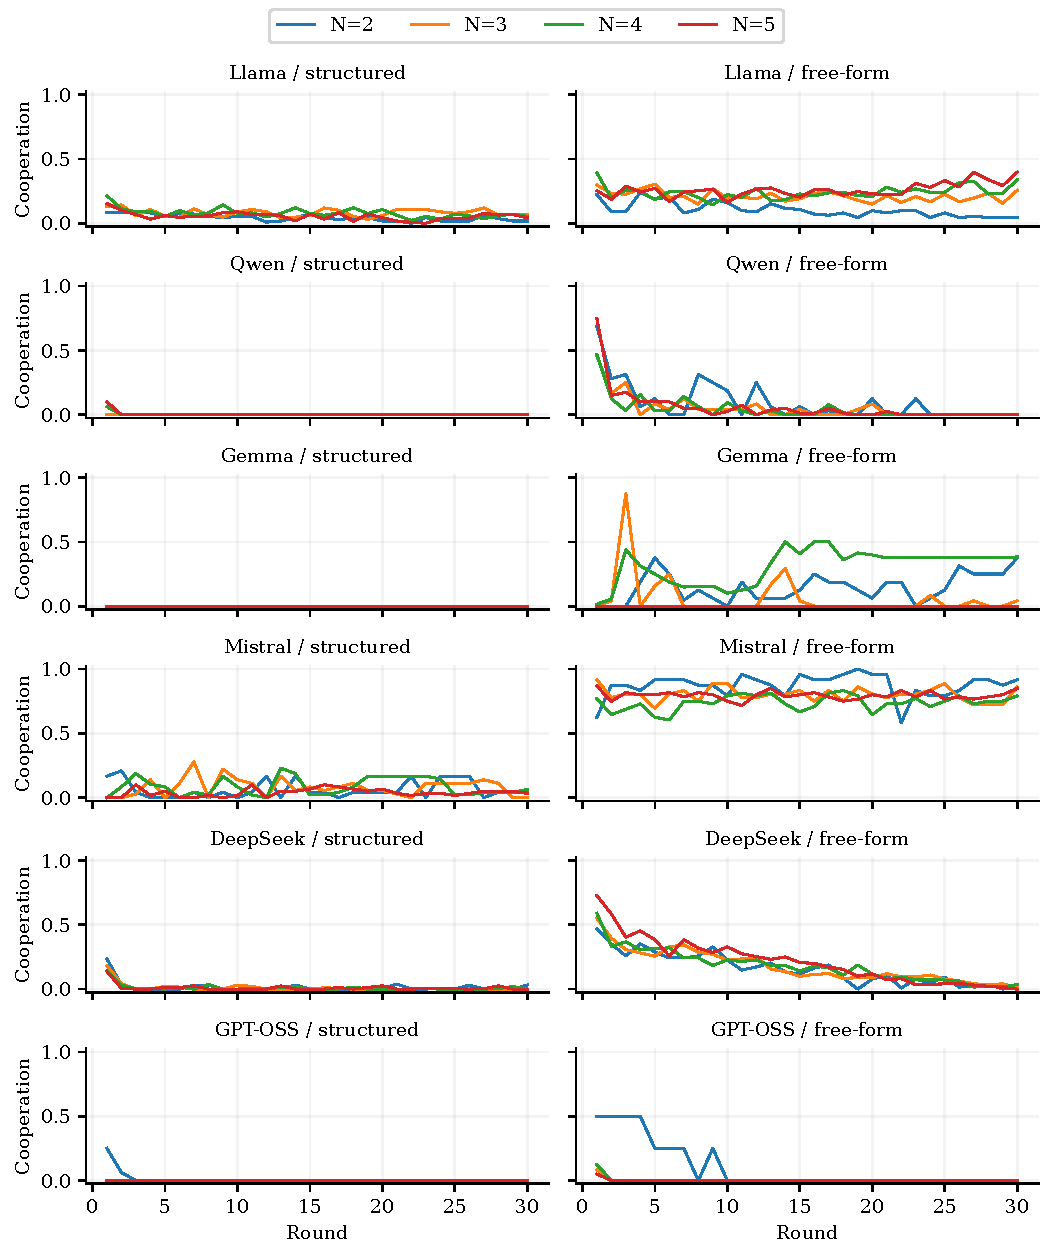
\includegraphics[width=0.9\textwidth]{main_trajectory_by_N.pdf}
\caption{Descriptive cell-mean trajectories by group size and mode. Curves average episodes within a cell across all 30 rounds. Group-size responses and persistence differ across models and scaffolds; these descriptive trajectories introduce no new tests.}
\label{fig:traj-by-N}
\end{figure*}

\section{Qwen Saved-Log Checks and Dataset Provenance}
\label{sec:qwen-log-check}
The primary Qwen results use 32 fresh main episodes, seeds 1001--1004, with four episodes in each mode-by-$N$ cell. The analyzed Qwen data match the full experiment export. The separate parser-v2 rerun, seeds 106--110, contains 35 pilot episodes (20 structured, 15 free-form), not a complete replacement main grid, and is not merged into the primary dataset.

These post-hoc checks use the saved main actions and original fallback flags, not new inference. Qwen free-form has 100 fallbacks among 1{,}680 decisions overall, but none among the 280 decisions in rounds 26--30, all of which have zero cooperation. This rules out direct fallback substitution as the source of late zero cooperation, without ruling out effects of earlier fallbacks on subsequent histories.

A first-attempt-valid check recomputes validity from each initial response with the v2 extractor and action validator. It reports free-form cooperation of 60.42\% in rounds 1--5 and 0.00\% in rounds 26--30, averaging eligible decisions within episodes and equally across the four group sizes. These conditional summaries retain the observed pipeline-generated histories; they are not trajectories from an intervention restricted to first-attempt decisions. Only one free-form episode has no fallbacks, and the missing retained cells prevent a complete filtered comparison. The saved-log checks therefore clarify fallback timing without establishing robustness across fallback-free episodes.

\section{Prompt Templates}
\label{sec:appendix-prompts}

The text below gives the shared system and condition-specific decision
instructions. Each decision also receives a JSON state containing the action
mapping, payoff and dynamics rules, current state, and observed histories.
Its \texttt{temporal\_context} explicitly supplies
\texttt{total\_rounds=30} and
\texttt{rounds\_remaining\_including\_current=31-t}.
Thus agents are informed of the finite horizon; the opening and final rounds
are not presented as an unknown-length interaction.

\paragraph{Base system prompt (both conditions).}
\begin{verbatim}
You choose an action in a repeated
multi-player game to maximize your own
long-term average reward. Use the
supplied individual observed
histories, action mapping, payoff
rules, and temporal context. Actions
are simultaneous. Other players'
current actions are unknown.
Distinguish observations from true
actions and tentative hypotheses from
evidence. You may form tentative
opponent-strategy hypotheses; do not
treat a label as evidence. No
particular action, cooperation level,
or amount of action switching is
preferred. Do not invent observations,
future responses, or missing rules.
Return one JSON object matching the
requested schema, without markdown.
\end{verbatim}

\paragraph{Free-form decision prompt.}
\begin{verbatim}
Choose one valid action using the
supplied evidence and objective.
Account for immediate rewards and any
future consequences justified by the
game rules and observed behavior.
Explain your reasoning, including how
you weighed the current game state and
history. Include opponent predictions
only when requested by the output
schema. The action must be an integer
in the supplied action space.
Additional reporting fields do not
determine action validity.
\end{verbatim}

\paragraph{Structured decision prompt.}
\begin{verbatim}
Choose one valid action using the
supplied evidence and objective.
Account for immediate rewards and any
future consequences justified by the
game rules and observed behavior.
Explain your reasoning, including how
you weighed the current game state and
history. Include opponent predictions
only when requested by the output
schema. You have been given a pre-
computed ranking of actions by
expected utility. Consider it
alongside your own reasoning; you are
not required to choose the top-ranked
action. The action must be an integer
in the supplied action space.
Additional reporting fields do not
determine action validity.
\end{verbatim}



\section{Post-hoc Timing and Explanation Descriptions}
\label{sec:log-descriptions}
These descriptions use only the original 376 completed episodes and saved
returned explanations; no new inference, semantic judge, human annotation,
or significance tests are used. All 39{,}480 saved per-seat inputs explicitly
contain the 30-round horizon and remaining-round count.

\paragraph{Thresholds and terminal zero cooperation.}
The first model--scaffold mean below .5 in Figure~\ref{fig:dynamics}
averages the four $N$ cells equally. It is round 1 for every structured
curve and for Llama, Gemma, and GPT-OSS free-form; it is round 2 for
Qwen and DeepSeek free-form, and never occurs for Mistral free-form.
This aggregate threshold marker is distinct from an episode's active
streak break: $g_t<.5$ with $s_{t-1}>0$. Round-1 floors are not breaks.
Recovery means reaching $g_t\geq.5$ within the next three available
rounds after the first active break. Terminal-zero onset is the first
round of an all-zero cooperation suffix ending at round 30; episodes
already at zero throughout are reported separately. A suffix beginning
at round 30 is a one-round endpoint observation, not evidence of a
longer collapse. Table~\ref{tab:log-timing} reports all models and modes;
counts use episodes, and medians condition on the event occurring.
No episode is removed from the primary analysis.
\begin{table*}[t]
\centering\small
\setlength{\tabcolsep}{3pt}
\begin{tabular}{llrrrrrrrr}
\toprule
Model & Mode & $n$ & Breaks & \shortstack{Break\\median $t$} & Recovery & Floors & Terminal & \shortstack{Onset\\median $t$} & Late \\
\midrule
Llama & S & 56 & 14 & 5 & 3 & 6 & 38 & 21 & 15 \\
Llama & F & 56 & 48 & 6 & 9 & 1 & 19 & 24 & 8 \\
Qwen & S & 16 & 0 & -- & 0 & 13 & 3 & 2 & 0 \\
Qwen & F & 16 & 12 & 2 & 2 & 0 & 16 & 18 & 0 \\
Gemma & S & 32 & 0 & -- & 0 & 32 & 0 & -- & 0 \\
Gemma & F & 32 & 17 & 4 & 8 & 10 & 12 & 20 & 4 \\
Mistral & S & 12 & 4 & 11 & 1 & 0 & 7 & 24 & 3 \\
Mistral & F & 12 & 1 & 22 & 1 & 0 & 0 & -- & 0 \\
DeepSeek & S & 64 & 15 & 2 & 0 & 12 & 51 & 15 & 8 \\
DeepSeek & F & 64 & 56 & 3 & 36 & 0 & 59 & 24 & 24 \\
GPT-OSS & S & 8 & 1 & 2 & 0 & 7 & 1 & 3 & 0 \\
GPT-OSS & F & 8 & 1 & 8 & 1 & 4 & 4 & 2 & 0 \\
\bottomrule
\end{tabular}
\caption{Post-hoc episode timing in the original cohort. S/F denote structured/free-form. Breaks count episodes with an active streak reset; Recovery counts return to $g_t\geq.5$ within the next three rounds after the first break. Floors are zero throughout all 30 rounds. Terminal counts episodes with an all-zero suffix beginning after round 1; Late counts these onsets in rounds 26--30. Medians condition on the respective event; dashes denote no events. Counts are descriptive and do not identify mechanisms.}
\label{tab:log-timing}
\end{table*}


\paragraph{Keyword definitions and denominators.}
We search the saved \texttt{reasoning\_text} field case-insensitively,
including explanations returned after repair. Ranking matches the literal
words \emph{rank}, \emph{ranks}, \emph{ranked}, \emph{ranking}, or the
phrase \emph{expected utility}. Horizon matches \emph{horizon},
\emph{end game}/\emph{end-game}, \emph{last round(s)},
\emph{final round(s)}, \emph{total round(s)},
\emph{round(s) remaining}, \emph{remaining round(s)},
\emph{round(s) left}, \emph{30-round}/\emph{thirty-round}
(also space-separated), or \emph{round 30}.
Generic references to future rewards are not counted as explicit horizon
mentions. Table~\ref{tab:log-keywords} reports percentages over all
seat-round decisions, including empty explanations as nonmatches;
nonempty counts expose this denominator choice. Rates weight decisions,
so larger groups contribute more text. They are descriptive lexical
frequencies, not estimates of strategy or validated explanation categories.
\begin{table*}[t]
\centering\small
\setlength{\tabcolsep}{3pt}
\begin{tabular}{llrrrrrr}
\toprule
Model & Mode & Decisions & Nonempty & Ranking $n$ & Ranking (\%) & Horizon $n$ & Horizon (\%) \\
\midrule
Llama & S & 5880 & 5801 & 5420 & 92.18 & 1604 & 27.28 \\
Llama & F & 5880 & 5705 & 2 & 0.03 & 1643 & 27.94 \\
Qwen & S & 1680 & 1665 & 874 & 52.02 & 104 & 6.19 \\
Qwen & F & 1680 & 1554 & 0 & 0.00 & 137 & 8.15 \\
Gemma & S & 3360 & 3360 & 3340 & 99.40 & 450 & 13.39 \\
Gemma & F & 3360 & 3360 & 0 & 0.00 & 545 & 16.22 \\
Mistral & S & 1260 & 1260 & 1067 & 84.68 & 294 & 23.33 \\
Mistral & F & 1260 & 1260 & 0 & 0.00 & 352 & 27.94 \\
DeepSeek & S & 6720 & 6692 & 3098 & 46.10 & 406 & 6.04 \\
DeepSeek & F & 6720 & 6641 & 0 & 0.00 & 732 & 10.89 \\
GPT-OSS & S & 840 & 840 & 142 & 16.90 & 228 & 27.14 \\
GPT-OSS & F & 840 & 834 & 0 & 0.00 & 215 & 25.60 \\
\bottomrule
\end{tabular}
\caption{Post-hoc literal keyword matches in returned explanations. Percentages use all seat-round decisions, including empty explanations as nonmatches; Nonempty reports the number with nonblank text. S/F denote structured/free-form. Categories may overlap. These decision-weighted lexical counts are not validated semantic labels, estimates of hidden reasoning, or independent behavioral replicates.}
\label{tab:log-keywords}
\end{table*}

\end{document}
